\documentclass[conference]{IEEEtran}

\usepackage[utf8]{inputenc}
\usepackage[T1]{fontenc}
\usepackage{graphicx}
\usepackage{amsmath}
\usepackage{amsfonts}
\usepackage{booktabs}
\usepackage{multirow}
\usepackage{siunitx}
\usepackage{xcolor}
\usepackage{cite}
\usepackage{url}
\usepackage{array}
\usepackage{caption}
\usepackage{subcaption}

\captionsetup{font=footnotesize}

\title{Efficient Annotation and Baseline Modeling for Littoral Marine Radar Object Detection and Classification}

\author{
\IEEEauthorblockN{Author Name}
\IEEEauthorblockA{
Department or Lab \\
Institution \\
Email: name@example.com}
}

\begin{document}

\maketitle

\begin{abstract}
Fixed-site littoral radar installations are increasingly attractive for low-cost monitoring of harbors, lakes, and coastal approaches, but supervised learning on such data remains bottlenecked by annotation effort. This paper presents an end-to-end system for transforming raw sweeps from a short-range X-band recreational marine radar into history-augmented polar images, and for efficiently annotating those images using a Rust/Slint front-end integrated with a CPU-only YOLO v12n pre-annotator. The radar is deployed at several littoral and inland-water sites, including Lake Murray, Lake Greenwood, Lake Monticello, multiple Charleston-area coastal locations, and Portsmouth City Park, yielding approximately thirty hours of data and about two hundred thousand scans. Each scan is converted into a \mbox{1735$\times$1735} polar history image that encodes several seconds of motion; targets are labeled into three classes (small vessel, large vessel, buoy) while all remaining returns are treated as background clutter or static land.

The annotation tool is explicitly designed for secure and resource-constrained environments: all pre-annotation runs on an Apple M1 Pro CPU, at approximately one second per full radar frame, without requiring a dedicated GPU server. A hyper-specialized YOLO v12n pre-annotator is fine-tuned for each dataset using one to five epochs of training over 160$\times$160 patches extracted from the polar images. A second, more extensively trained YOLO v12n model provides baseline detection performance on the labeled dataset. The paper describes the radar hardware and installation sites, the radar-to-image conversion pipeline, the annotation interface and pre-annotation strategy, and baseline detection experiments on early labels and on an expanded dataset expected to reach approximately one thousand labeled frames. Sensitivity to temporal history length and to the number of labeled frames is analyzed, providing practical guidance for littoral radar projects that must operate with limited annotation budgets and CPU-only resources.
\end{abstract}

\begin{IEEEkeywords}
Marine radar, object detection, littoral sensing, annotation tools, YOLO, polar images.
\end{IEEEkeywords}

\section{Introduction}

Littoral environments such as harbors, inlet channels, and nearshore waterways are challenging for radar-based perception. Short-range recreational marine radars provide inexpensive, widely available X-band sensing, but their returns in littoral regimes are dominated by land reflections, piers and jetties, static structures, and complex multipath. This degradation is compounded by sparse and low-SNR signatures from small craft, buoys, and kayaks, which are often the very objects of interest for safety and situational awareness. Supervised learning systems for such data require carefully curated labels, yet the annotation of radar images remains difficult and time-consuming, particularly when standard vision tools designed for RGB images are used without adaptation.

This work focuses on fixed-site deployments of a recreational X-band marine radar at several littoral and inland-water locations. The radar is operated primarily at 1--2\,NM range, with a maximum configured range of 3\,NM. The antenna is installed on piers, towers, and shore structures at heights ranging from approximately \SI{7}{ft} to \SI{30}{ft} above the water surface, depending on the local elevation and mounting geometry. Sites include Lake Murray dam, Lake Greenwood State Park, Lake Monticello, multiple coastal locations near Charleston, SC (Folly Beach, Grice Marine Lab, Demetre Park), and Portsmouth City Park in Virginia. These sites span quiet lakes, busy harbors, and strongly cluttered coastal scenes.

The first goal of the paper is to describe a practical pipeline that converts raw shore-based radar sweeps into history-augmented polar images suitable for both human annotation and training of convolutional object detectors. The second goal is to present an annotation environment tailored to littoral radar imagery, implemented in Rust with a Slint user interface, and tightly coupled to a CPU-based YOLO v12n pre-annotator. The third goal is to provide baseline detection results on the emerging dataset and to study the sensitivity of those results to temporal history length and dataset size.

The contributions of this paper can be summarized as follows. A complete radar-to-image converter is described for short-range X-band recreational radar at fixed littoral sites, including polar representation, temporal history encoding over several seconds, and basic masking of static land returns. A Rust/Slint annotation front-end is introduced that runs entirely on MacOS in secure, GPU-less environments, integrates a hyper-specialized CPU-based YOLO v12n pre-annotator, and supports point, bounding-box, and segmentation modes tailored to marine targets. A dataset of approximately thirty hours of radar recordings from seven sites is characterized, together with an emerging labeled subset expected to reach about one thousand frames, using a three-class taxonomy covering small vessels, large vessels, and buoys. Baseline YOLO v12n detection experiments are reported on early labels (approximately two hundred frames) and on the expanded dataset, including sensitivity to history length and to the number of labeled frames.

The remainder of the paper is organized as follows. Section~\ref{sec:related} reviews related work on marine radar datasets, radar image representations, and annotation systems. Section~\ref{sec:data} details the radar hardware, sites, collection protocol, and radar-to-image generation. Section~\ref{sec:annotation} presents the annotation system design, including the Rust/Slint interface and YOLO pre-annotator. Section~\ref{sec:methods} describes the experimental methodology for baseline detection models and sensitivity studies. Section~\ref{sec:results} reports experimental results. Section~\ref{sec:discussion} discusses implications, and Section~\ref{sec:conclusion} concludes with future work.

\section{Related Work}
\label{sec:related}

Research on marine radar perception has explored both commercial and recreational radar units for vessel detection, tracking, and classification in open-sea and coastal environments. Commercial navigational radars often provide higher power, narrower beamwidth, and proprietary processing pipelines, whereas recreational units are widely available but more constrained in dynamic range and configurable processing. Several public datasets and studies have focused on conventional marine radars mounted on vessels or offshore platforms; fewer works consider fixed-site shore-based deployments in shallow or cluttered littoral zones and lakes.

Radar image representations for maritime scenes vary from raw polar-range-azimuth grids, through Cartesian reprojections, to learned feature maps. Polar images preserve the native sampling and angular resolution of the radar, at the cost of non-uniform spatial resolution with range. Cartesian reprojection simplifies integration with optical imagery and geographic information systems but can introduce interpolation artifacts and distort targets at long range. For littoral scenes where the primary interest is within a few nautical miles, polar representations provide a convenient compromise that avoids reprojection and preserves the structure of azimuthal sweeps.

Annotation tools for radar and sonar differ from general-purpose image labelers in several respects. The expected target sizes, intensities, and shapes often require magnified views, specialized colormaps, and temporal context for disambiguation. Some prior systems for sonar and specialized radar have introduced domain-aware interfaces, but many practitioners still rely on generic tools such as Label Studio, CVAT, or LabelImg, which were designed for RGB photographs and do not integrate tightly with radar-specific pre-annotation pipelines or polar coordinate systems.

Auto-labeling and semi-automatic methods have been investigated in the broader vision community, including detector-based pre-annotation, active learning, and semi-supervised learning. In many of these systems, pre-annotation is performed on powerful GPU servers and pushed to client interfaces as a service. The setting considered here is deliberately different: annotations must be performed on secure MacOS laptops, without network-connected GPU backends, and therefore require a CPU-only pre-annotation pipeline that remains usable at interactive latencies. This constraint shapes the design choices described in the following sections.

\section{Littoral Radar Data and Image Generation}
\label{sec:data}

\subsection{Radar System and Site Installation}

The sensing hardware is a recreational Furuno-class X-band marine radar system. The radar operates at X-band with a maximum configured range of approximately 3\,NM. In the deployments considered here, the range is typically set to 1 or 2\,NM, since the areas of interest are harbor approaches, nearshore channels, and lake surfaces relatively close to shore. Range and azimuth resolutions follow manufacturer specifications for this class of radar; beamwidth is characteristic of small recreational antennas, and the antenna rotation rate corresponds to a sweep period on the order of several seconds.

Installations are at fixed shore sites. The antenna is mounted on piers, towers, and park structures such that the physical height above the mounting platform is approximately \SI{5}{ft}. The resulting antenna height above the water surface ranges from roughly \SI{7}{ft} to \SI{30}{ft}, depending on the local ground elevation at each site. The sites include Lake Murray dam and Lake Greenwood State Park, which provide reservoir environments with controlled shorelines; Lake Monticello, which offers another inland water body; Folly Beach, Grice Marine Lab, and Demetre Park in the Charleston area, which contribute coastal and tidal environments; and Portsmouth City Park in Virginia, which adds a harbor-like setting with man-made structures.

Figure~\ref{fig:sitesmap} illustrates the geographic distribution of these sites and includes representative photographs of several installations. This diversity is intended to cover quiet lakes, moderately busy waterways, and more complex coastal clutter.

\begin{figure}[t]
    \centering
    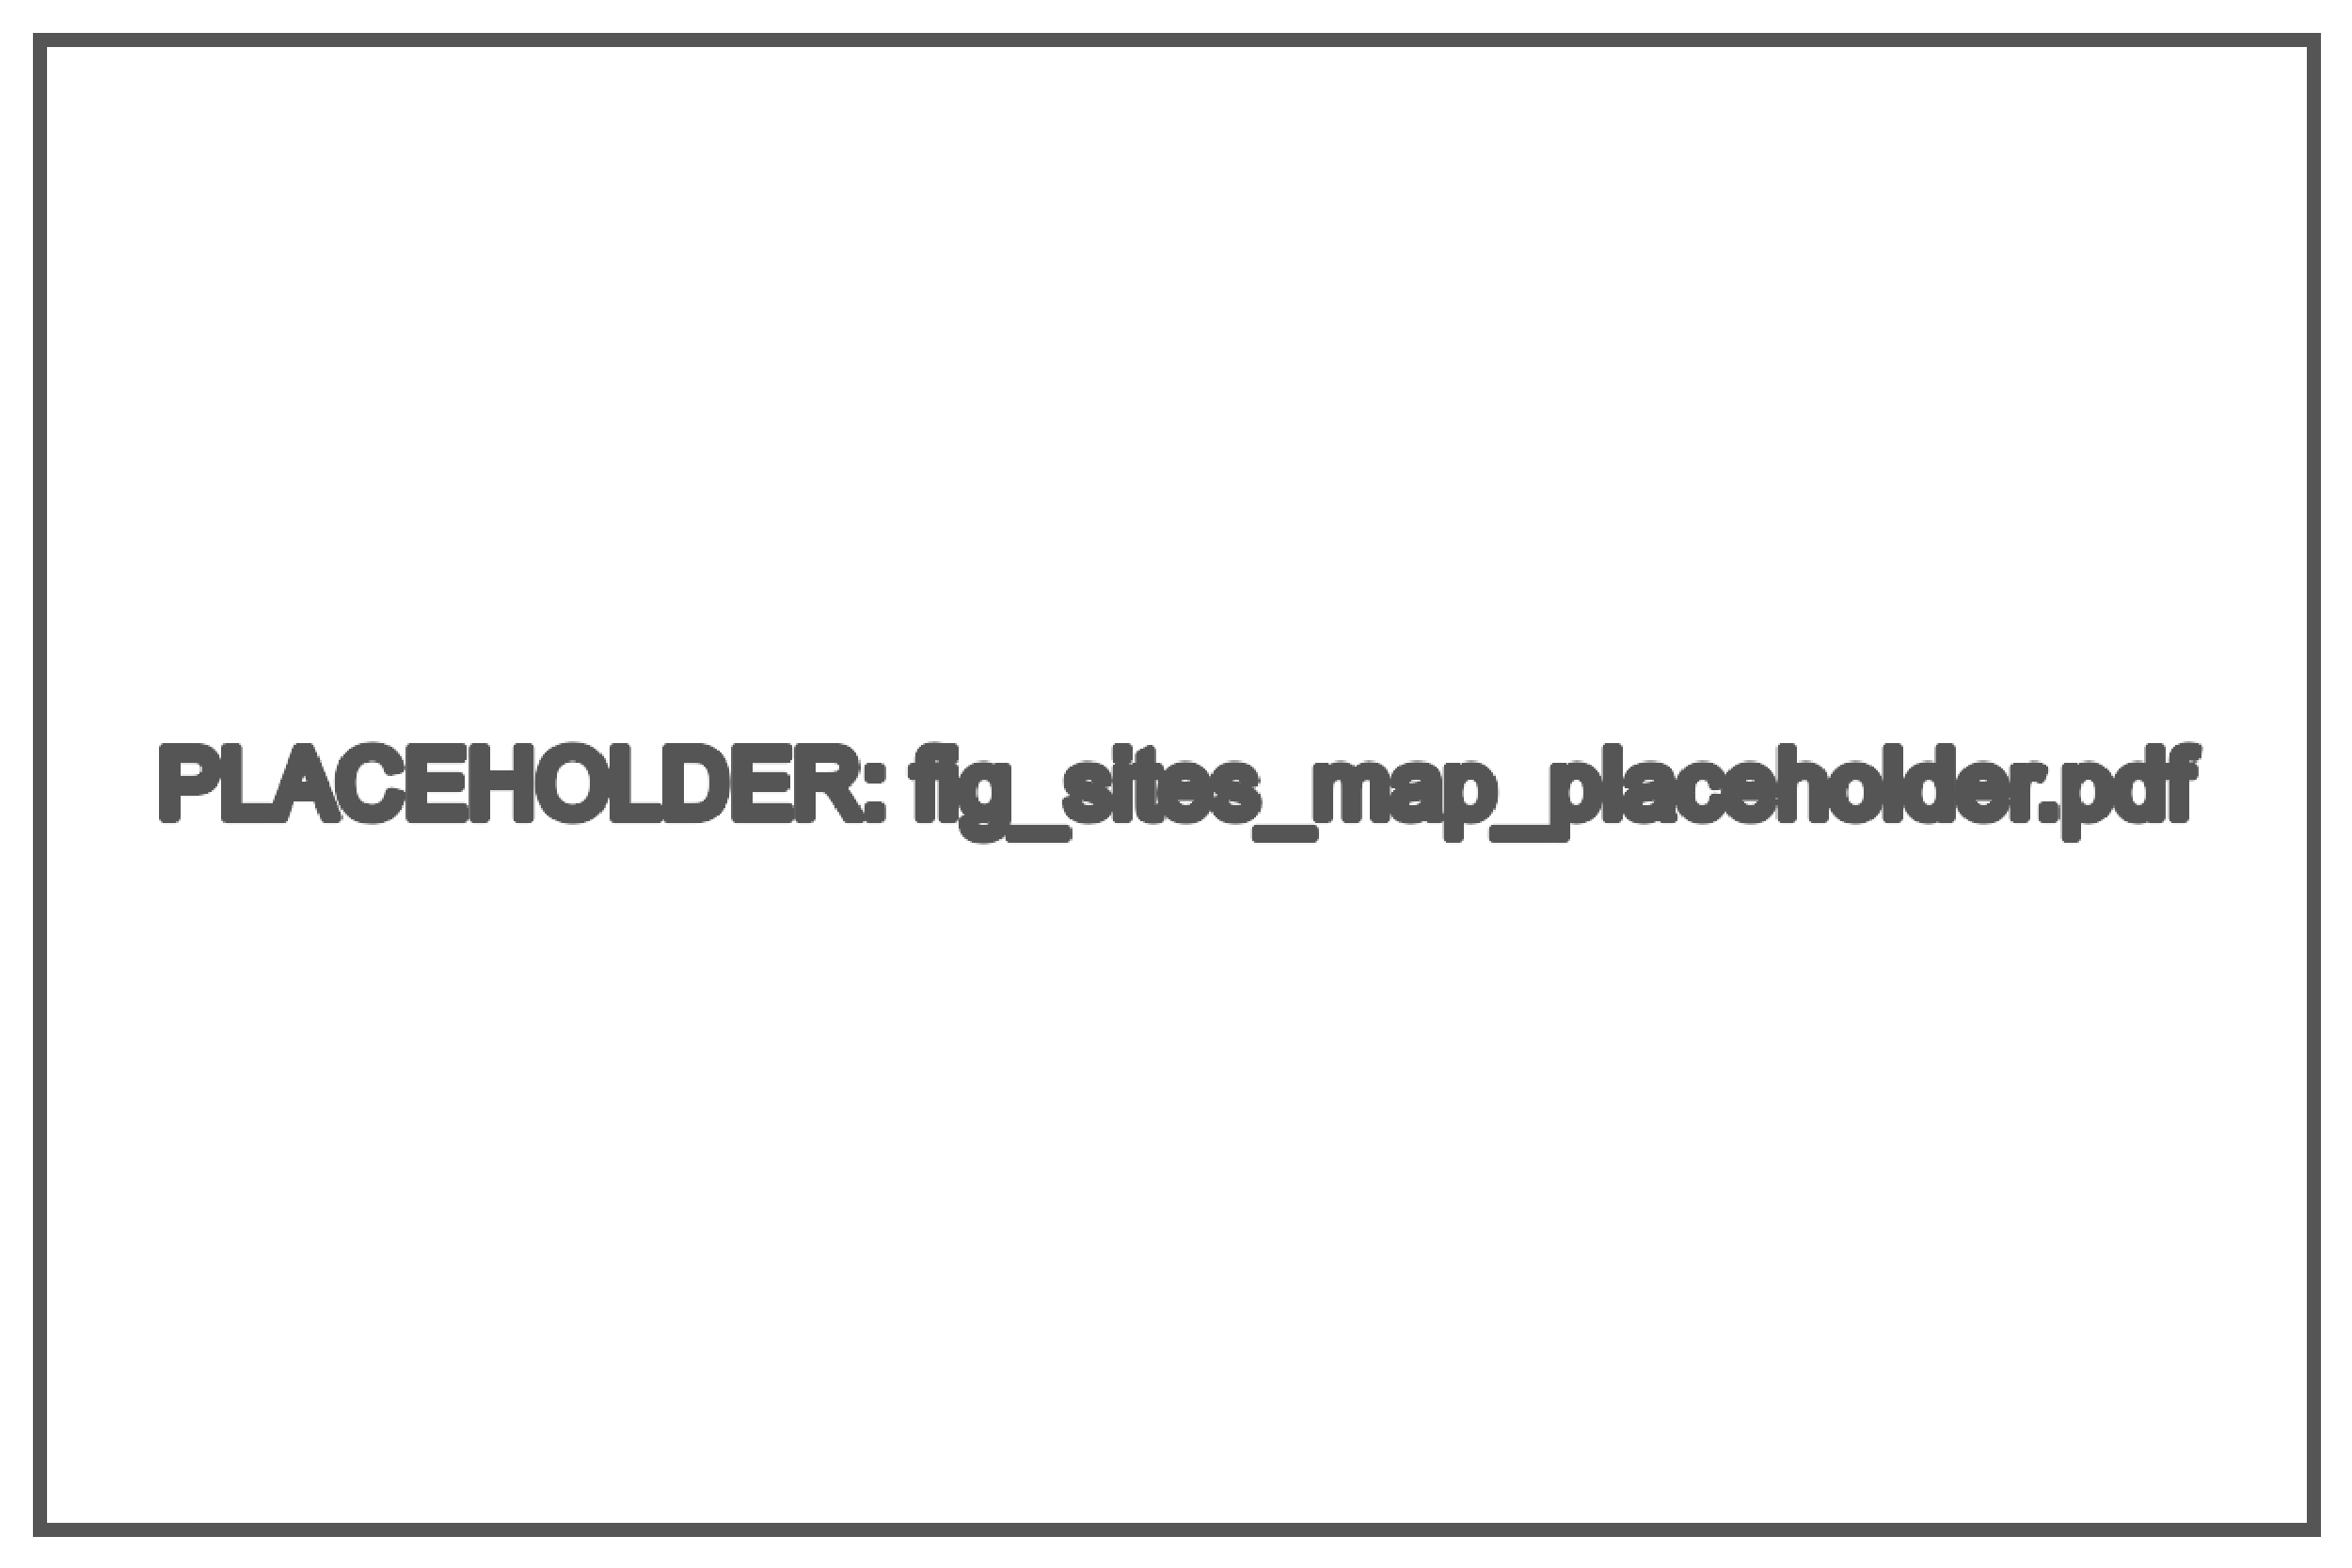
\includegraphics[width=\linewidth]{fig_sites_map_placeholder.pdf}
    \caption{Deployment locations for the fixed-site littoral radar installations, including inland lakes and coastal or harbor environments. Site photographs illustrate antenna mounting heights and surrounding geometry.}
    \label{fig:sitesmap}
\end{figure}

\subsection{Littoral Data Collection Protocol}

Data collection is conducted by operating the radar continuously over multi-hour sessions at each site. Across all locations, the current dataset comprises approximately thirty hours of recordings and about two hundred thousand individual scans or frames. Sessions are scheduled to capture a range of environmental and traffic conditions, including daytime and nighttime periods, differing wind and wave states, various tide levels at coastal sites, and both low and moderate vessel traffic.

The operating area for each site is defined by the radar range configuration and local geometry. For lake sites, the area of interest is usually the open water in front of dams, boat ramps, or recreational channels. For coastal sites such as Folly Beach and the Charleston locations, the area includes nearshore surf zones, inlets, and navigation channels where small craft, buoys, and shoreline structures coexist. At Portsmouth City Park, the area includes piers, moored vessels, and nearby channels.

Site logs record the start and end times of each collection, radar configuration such as range setting, and notable events such as changes in weather or traffic. These logs are synchronized with the radar data stream using timestamps and are used later to select labeling subsets.

\subsection{Signal Processing and Radar-to-Image Converter}

The radar-to-image converter transforms raw radar sweeps into history-augmented polar images suitable for display and machine learning. Each scan is represented in a polar grid indexed by range bin and azimuth bin. The base representation preserves this polar structure without reprojection to Cartesian coordinates, resulting in images of size \mbox{1735$\times$1735} pixels for the current configuration.

Temporal history is encoded by aggregating multiple scans over a fixed time window. The default configuration aggregates approximately six seconds of radar history, which corresponds to several antenna rotations depending on the rotation rate. A temporal decay is applied so that more recent scans contribute more strongly to the intensity of each pixel, while older scans are down-weighted. This history encoding emphasizes moving targets and smooths out some of the stochastic variability in individual sweeps.

The number of history frames is treated as a tunable parameter and is later varied in sensitivity experiments. Shorter histories can reduce smearing of fast-moving vessels and maintain sharper responses, while longer histories can help integrate weak returns from small or intermittently visible targets. In all cases, the history-encoded image for each time step can be generated essentially instantaneously once the raw sweeps are available, since the aggregation is a simple accumulation with decay and the implementation is optimized for the fixed polar grid.

Static land and large man-made structures introduce strong, persistent returns that dominate the dynamic range. In the current system, these regions are treated as background and are handled primarily by the training process and the label taxonomy, rather than by aggressive clutter suppression. Static masking of land is applied where reliable shoreline maps are available, but the focus of this paper is on the annotation and modeling pipeline, not on developing advanced clutter suppression algorithms.

Figure~\ref{fig:historyimages} shows example history-encoded polar images from clean lake conditions and from heavily cluttered coastal scenes, illustrating the dynamic range and interference patterns that annotators must interpret.

\begin{figure}[t]
    \centering
    \includegraphics[width=\linewidth]{fig_history_examples_placeholder.png}
    \caption{Example \mbox{1735$\times$1735} polar history images. Top: relatively clean lake scene with a small number of vessels. Bottom: cluttered coastal scene with strong land returns, piers, and multiple moving targets.}
    \label{fig:historyimages}
\end{figure}

\subsection{Dataset Description}

Table~\ref{tab:dataset} summarizes the current dataset. Approximately thirty hours of recordings yield around $2\times 10^5$ scans, each converted into a history-encoded polar image. Labeled data collection is ongoing; at the time of writing, fewer than two hundred frames have been labeled, with an expected total of about one thousand labeled frames by the time of presentation.

The label taxonomy assigns each target to one of three classes: small vessel, large vessel, and buoy. The intention is that small vessels include small motorboats, personal watercraft, kayaks, and similar craft with relatively small radar cross-sections, while large vessels include larger motor vessels and commercial craft with larger signatures. Buoys include navigation markers and moored buoys that appear as localized, mostly static returns. All other returns, including land, piers, unidentified clutter, and unlabelled targets, are treated as background. No special rules are imposed regarding ghost reflections or multipath; ambiguous or low-confidence returns that do not clearly fall into the three classes are left unlabeled.

\begin{table}[t]
    \centering
    \caption{Summary of current littoral radar dataset}
    \label{tab:dataset}
    \begin{tabular}{p{0.55\linewidth}r}
        \toprule
        Quantity & Value \\
        \midrule
        Total recording time & $\approx 30$\,h \\
        Number of scans / frames & $\approx 200{,}000$ \\
        Image resolution & $1735 \times 1735$ polar \\
        Current labeled frames & $< 200$ \\
        Target labeled frames (by presentation) & $\approx 1000$ \\
        Classes & small vessel, large vessel, buoy \\
        Sites & 7 (lakes, coastal, harbor) \\
        \bottomrule
    \end{tabular}
\end{table}

\section{Annotation System Design for Littoral Radar}
\label{sec:annotation}

\subsection{System Overview and Data Flow}

The annotation system is designed as an end-to-end pipeline that starts from raw radar sweeps and ends with label files suitable for training and evaluating detection models. Raw polar scans are first converted into history-encoded \mbox{1735$\times$1735} images as described in Section~\ref{sec:data}. These images are stored in a format that preserves timestamps and is easily accessible from the Rust/Slint front-end, such as a directory of image files accompanied by metadata in a lightweight database or JSON-based index.

For each image, a CPU-based YOLO v12n pre-annotator can be invoked to produce initial bounding boxes and class predictions. Pre-annotations for all images in a labeling batch are generated in the background on the same MacOS machine that runs the front-end, at approximately one second per full frame. The pre-annotations are stored alongside the images in the same directory or database structure.

The Rust/Slint annotation interface then loads the images and their corresponding pre-annotations. Annotators review and edit these suggestions, add new annotations where needed, and decide whether to use point, bounding box, or segmentation modes. Once a set of frames is annotated, the labels are exported in a format compatible with YOLO training, including normalized bounding boxes and class indices. Quality-control metadata and timing logs are also exported.

Figure~\ref{fig:pipeline} depicts this data flow from radar to labels and back to model training.

\begin{figure}[t]
    \centering
    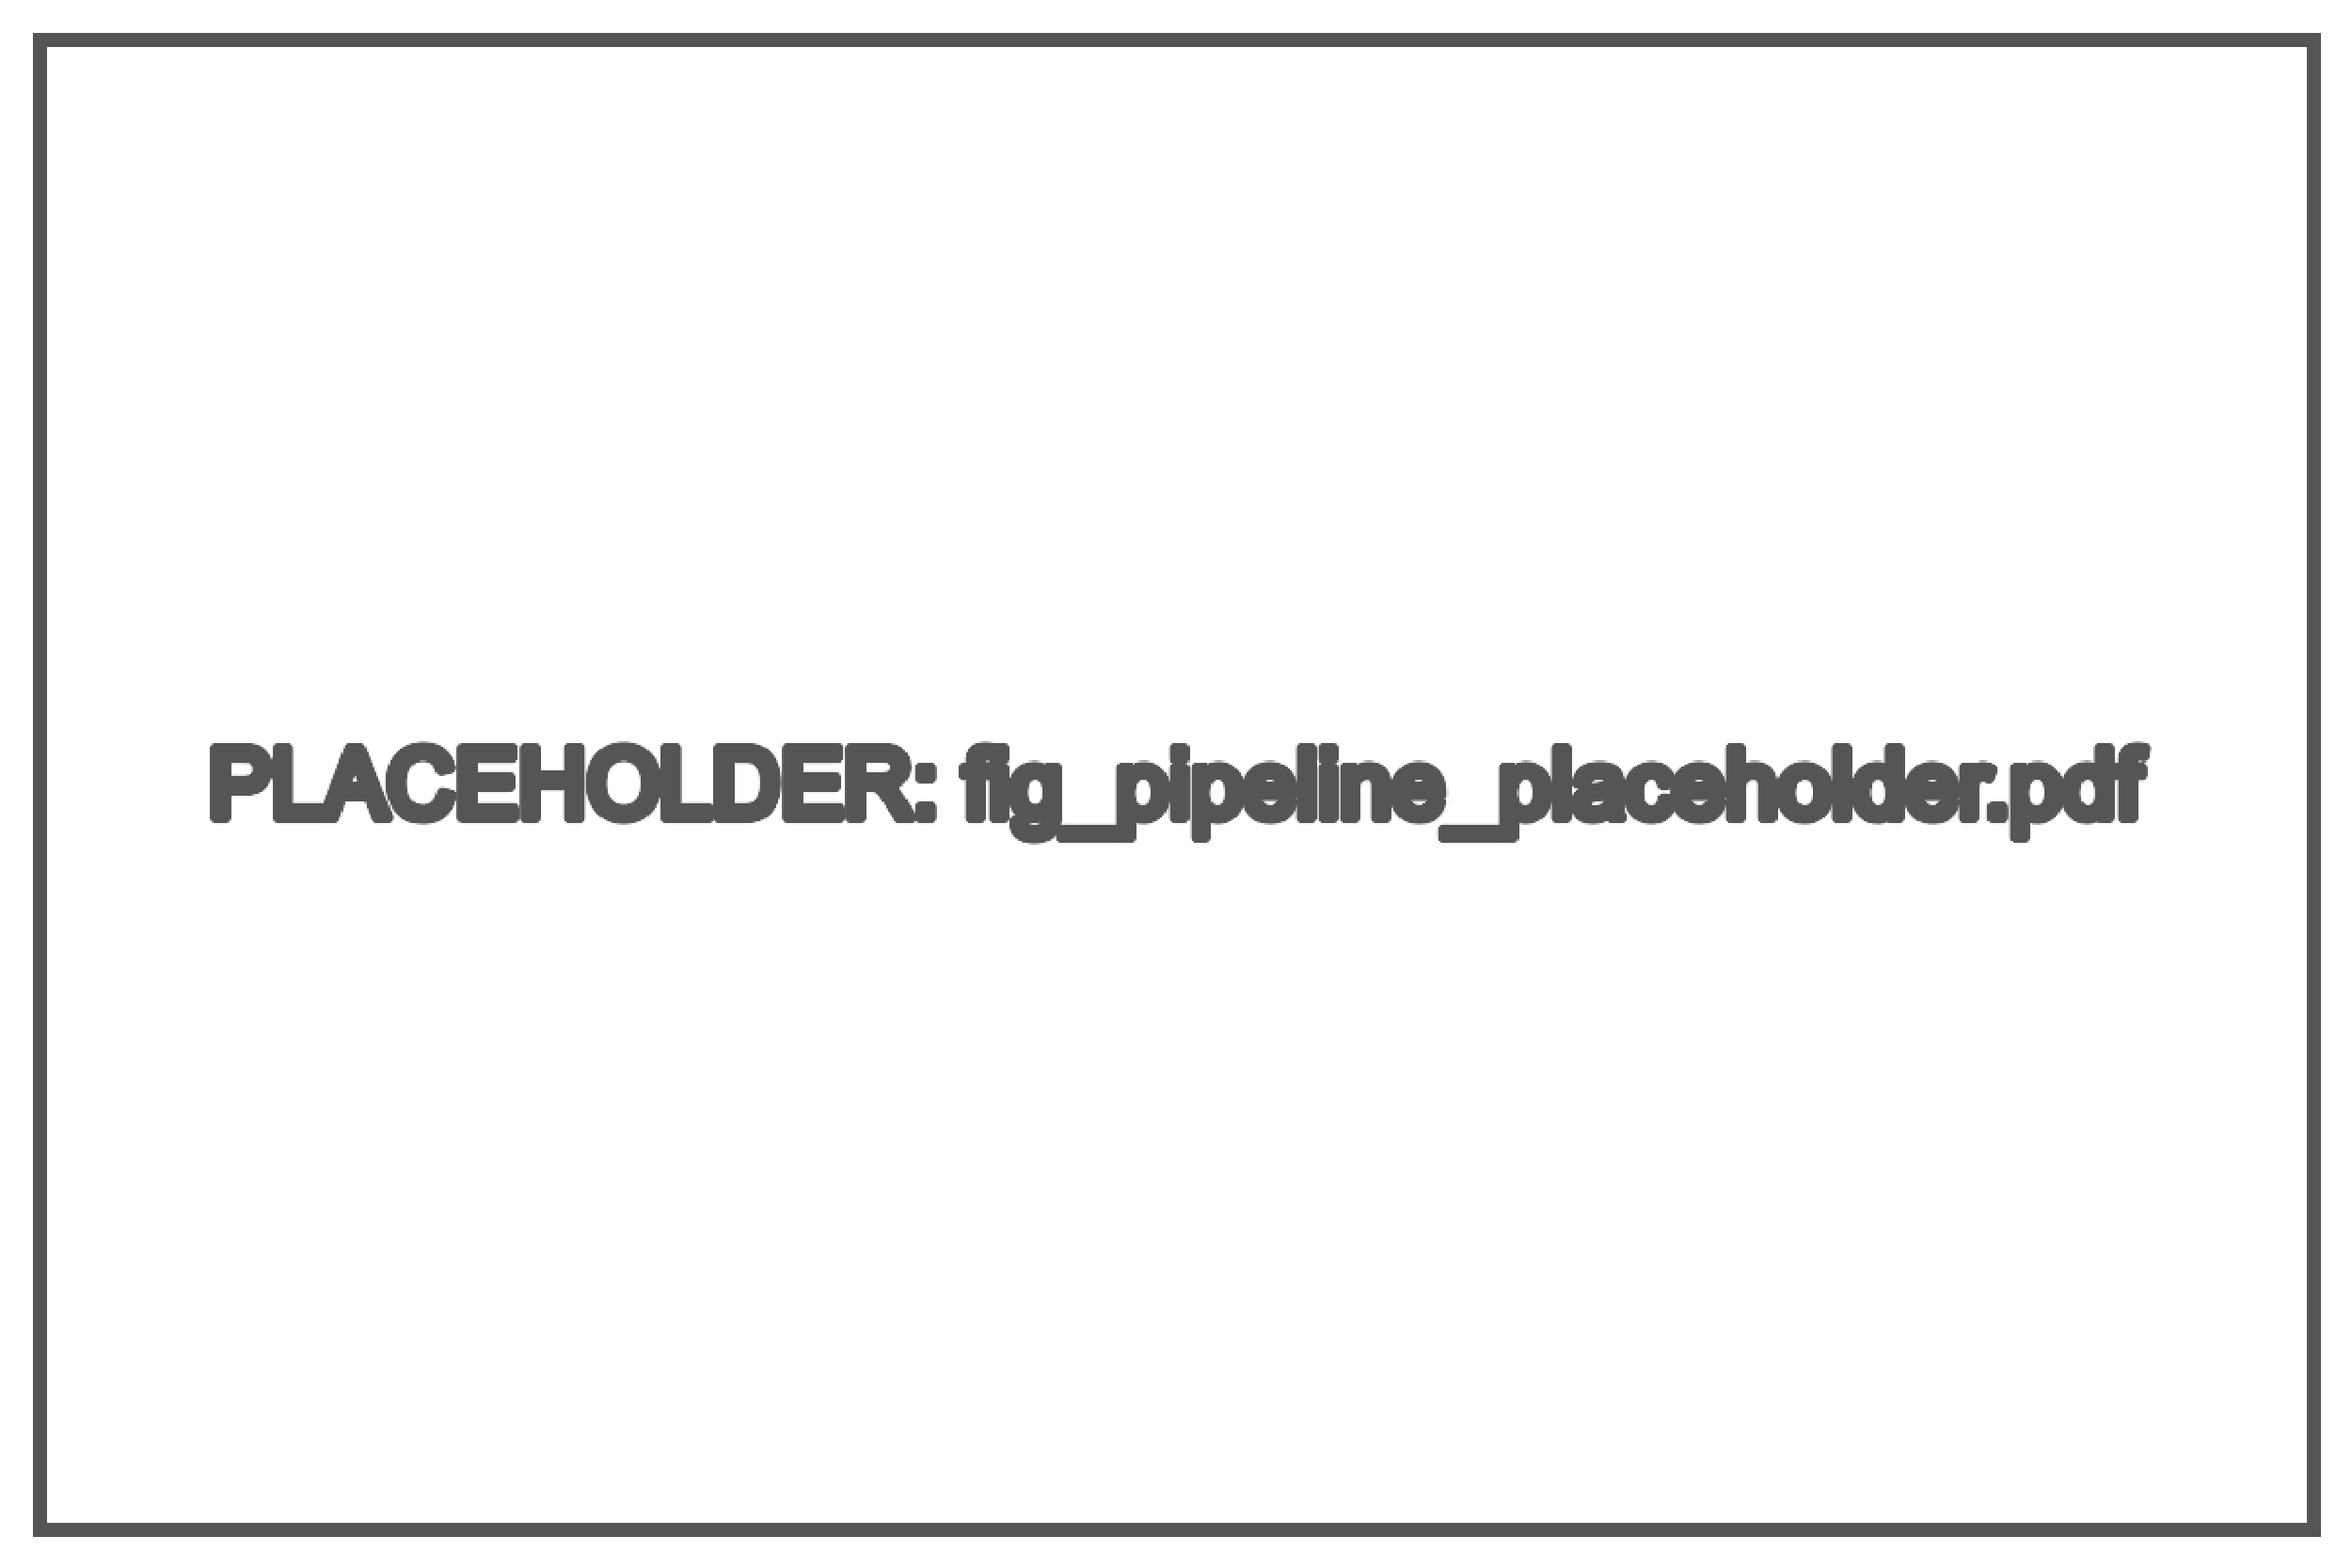
\includegraphics[width=\linewidth]{fig_pipeline_placeholder.pdf}
    \caption{System pipeline from raw radar sweeps to history-encoded polar images, CPU-based YOLO v12n pre-annotations, Rust/Slint annotation interface, and final labels used for training baseline detection models.}
    \label{fig:pipeline}
\end{figure}

\subsection{Rust/Slint Labeling Interface}

The annotation front-end is implemented in Rust with a Slint user interface and runs on MacOS laptops. This design choice reflects the need to operate in secure environments without external GPU servers or network dependencies and to maintain a small, easily auditable code base.

The interface presents history-encoded polar images with a colormap and intensity scaling that emphasizes vessel and buoy returns. Annotators can pan and zoom, switch between frames, and toggle overlays such as pre-annotations, existing labels, and optional land masks. Keyboard shortcuts and mouse interactions are chosen to minimize friction: common operations such as accepting or rejecting pre-annotations, drawing new boxes, adjusting box extents, and switching classes are bound to single keys or simple combinations.

The interface was developed with pre-annotation at its core. Rather than retrofitting pre-annotations onto a generic box-drawing workflow, the design assumes that many targets will already have YOLO-generated candidates. Annotators therefore spend more time confirming and refining boxes than drawing from scratch. This affects layout decisions, such as placing the list of pre-annotations prominently and providing rapid ways to navigate between them.

For comparison and context, Figure~\ref{fig:ui} contrasts the custom Rust/Slint interface with an earlier Label Studio based workflow. In the latter, radar images were treated as standard photographs, pre-annotations were not smoothly integrated, and GPU-backed pre-annotation services would have been required for real-time use. The custom tool avoids these dependencies and optimizes interaction for littoral radar.

\begin{figure}[t]
    \centering
    \begin{subfigure}{0.48\linewidth}
        \centering
        \includegraphics[width=\linewidth]{fig_slint_ui_placeholder.png}
        \caption{Rust/Slint tool}
    \end{subfigure}\hfill
    \begin{subfigure}{0.48\linewidth}
        \centering
        \includegraphics[width=\linewidth]{fig_labelstudio_ui_placeholder.png}
        \caption{Label Studio baseline}
    \end{subfigure}
    \caption{Annotation interfaces. The Rust/Slint tool on MacOS is designed around polar radar imagery and integrated pre-annotations, whereas a generic tool such as Label Studio treats radar frames as standard images and does not optimize for radar-specific workflows.}
    \label{fig:ui}
\end{figure}

\subsection{CPU-Based YOLO Pre-Annotator}

The pre-annotation component is a YOLO v12n detector configured for marine targets. It is initialized from a YOLO v8 model pretrained on standard vision datasets and then fine-tuned on the radar dataset. To accommodate the constraints of running on an Apple M1 Pro CPU, inference and training are performed on 160$\times$160 patches rather than on full-resolution images.

Each \mbox{1735$\times$1735} polar image is divided into patches that cover the image in an approximately $12\times 12$ grid. Patches near the boundaries are cropped or padded as needed to achieve consistent 160$\times$160 inputs. During training, each patch becomes an independent training sample. During inference, detections from overlapping patches are projected back into the coordinate frame of the full polar image and merged.

The pre-labelling model is designed to be hyper-specific to the current dataset and to adapt as more labeled data becomes available. For each dataset or labeling batch, the system runs a background fine-tuning job that trains the YOLO v12n model for one to five epochs on the currently available labeled patches. In many cases, one to three epochs are sufficient, with five epochs used as an upper bound to avoid overfitting and excessive training time. The resulting model is then used to pre-annotate frames in subsequent labeling batches.

On an Apple M1 Pro CPU, pre-annotation takes approximately one second per full \mbox{1735$\times$1735} frame, including all $12\times 12$ patches and post-processing to map detections back to the full image. This throughput allows annotators to work interactively with pre-annotations without a dedicated GPU server.

The confidence threshold for accepting predictions is configurable and exposed to the user. Annotators can trade recall against precision by adjusting this threshold within the front-end. No additional post-processing such as class remapping or custom non-maximum suppression beyond the standard YOLO NMS is currently applied; the design emphasizes simplicity and transparency.

\subsection{Annotation Modes in Maritime Scenes}

The tool supports three annotation modes that correspond to different types of targets and regions. Point annotation is intended for small or ambiguous radar returns where precise extents are not meaningful or where the target is effectively point-like at the radar resolution. Bounding box annotation is used for vessels and larger structures for which object detectors are expected to output bounding boxes and for which spatial extent matters. Segmentation annotation is reserved for extended regions such as land masses, piers, and large clutter fields when such regions are explicitly modeled.

In the current experiments, bounding boxes are the primary representation for small and large vessels and buoys. Point annotations may be used for very small or intermittent returns, but the main detection models are trained on bounding boxes derived from either boxes or translated points. Segmentation masks are not yet exploited for training, though the system is designed to support them in future work.

\subsection{Quality Control, Logging, and Export}

The front-end records metadata and timing information for each annotation. Timestamps are associated with frame loading, pre-annotation display, and commit operations when labels are saved. These logs enable later analysis of annotation effort, although this paper focuses on modeling results rather than human-efficiency metrics.

Exported labels include, for each bounding box, the frame identifier, class label, normalized center coordinates, width, and height in the YOLO format. Additional metadata such as annotator identity, confidence notes, and flags for difficult scenes can be stored in separate files or in extended formats. The export process is designed to be scriptable so that incremental batches of labels can be integrated into training pipelines with minimal manual intervention.

\section{Experimental Methodology}
\label{sec:methods}

\subsection{Pre-Annotation Training Protocol}

The pre-annotation YOLO v12n model is fine-tuned on the available labeled radar patches using a lightweight training schedule. For each new batch of labeled frames, all 160$\times$160 patches containing at least one labeled object are extracted. Negative patches containing only background are also sampled to control the class distribution. The patches are randomly shuffled and split into training and validation subsets.

Fine-tuning is performed for one to five epochs on this patch dataset, with the exact number chosen based on convergence diagnostics and the desired latency between labeling and updated pre-annotations. In many cases, one to three epochs suffice to obtain useful pre-annotations; five epochs are used as an upper bound. Data augmentation such as random flips, minor rotations, and intensity scaling is applied to improve robustness without significantly distorting the radar structure.

The training runs entirely on the Apple M1 Pro CPU used for annotation. The small model size of YOLO v12n and the modest number of epochs keep training times manageable, aligning with the design goal of a per-dataset, hyper-specific pre-annotator.

\subsection{Baseline Detection Model Training}

A separate YOLO v12n model is trained to provide baseline detection performance for evaluation. This model shares the same architecture and patch-based input format as the pre-annotator, but uses a more extensive training schedule and is not constrained to the minimal latency requirements of interactive annotation.

For the initial baseline, approximately two hundred labeled frames are used, split into 160 training frames and 40 validation frames in a random frame-wise split. As labeling progresses, the dataset is expected to grow to roughly one thousand labeled frames; the same 80/20 split strategy can be applied, yielding 800 training frames and 200 validation frames. For each frame in the training set, 160$\times$160 patches are extracted as in the pre-annotation pipeline.

Training is performed with standard YOLO optimization settings. A typical configuration uses a batch size chosen to fit within CPU memory constraints, an SGD or Adam optimizer with an initial learning rate on the order of $10^{-3}$, and a training schedule of, for example, 50--100 epochs when using the full dataset. Stronger augmentation can be applied than in the pre-annotation setting, including random cropping of patches, mild geometric distortions, and varying intensity transformations, since the goal is robust generalization across scenes and conditions.

The split is performed randomly by frame rather than by site in the initial experiments. This choice simplifies the analysis and ensures that both training and validation sets include frames from multiple sites. Future work can explore site-wise splits to assess cross-site generalization.

\subsection{Evaluation Metrics}

Detection performance is evaluated using standard object detection metrics adapted to the three-class marine taxonomy. For each class (small vessel, large vessel, buoy), average precision (AP) is computed at an intersection-over-union threshold of 0.5 between predicted and ground-truth bounding boxes. The mean average precision across classes, mAP@0.5, summarizes overall detection quality.

In addition to AP and mAP@0.5, per-class precision and recall are reported at one or more confidence thresholds. These metrics help characterize the trade-off between missed detections (false negatives) and false alarms (false positives), which is critical in safety-relevant littoral monitoring. F1 scores can also be derived from precision and recall for each class.

For some analyses, particularly those involving sensitivity to history length or dataset size, aggregated metrics such as overall recall for any target class and combined vessel detection performance (small and large vessels merged) may be reported to provide a simpler high-level view.

\subsection{Experimental Configurations}

Two main experimental axes are considered. The first axis is the amount of labeled data used for training the baseline detection model. Early experiments use the initial subset of approximately two hundred labeled frames (160 train, 40 val). Later experiments repeat the training procedure with the expanded dataset of approximately one thousand labeled frames (800 train, 200 val). Comparing these configurations reveals how detection performance scales with additional labels.

The second axis is the temporal history length used in the radar-to-image conversion. The default history window of approximately six seconds is compared against shorter and longer windows, for example three seconds and ten seconds, while holding other parameters fixed. This sensitivity study assesses whether shorter histories improve localization of fast-moving targets or whether longer histories strengthen weak returns from small vessels and buoys.

For each configuration, the same YOLO v12n architecture, patch extraction, and training hyperparameters are used. Differences in performance can therefore be attributed to the number of labeled frames and to the history length.

\section{Results}
\label{sec:results}

\subsection{Pre-Annotation Performance}

The pre-annotator achieves a throughput of approximately one second per full \mbox{1735$\times$1735} image on an Apple M1 Pro CPU, including processing of all 160$\times$160 patches and merging of detections. This latency is compatible with interactive use in the annotation interface, allowing annotators to load frames that have been pre-annotated just in time.

Qualitative inspection of pre-annotations shows that, after one to three epochs of fine-tuning on the current dataset, the model reliably proposes bounding boxes for medium and large vessels and many buoys, even in cluttered scenes. False positives occur near strong land reflections and piers, particularly when history length is long enough to smear static structures. In these cases, annotators can quickly reject erroneous boxes.

Figure~\ref{fig:preannots} illustrates typical pre-annotation outputs. Accepted boxes are shown along with ground-truth annotations after human review, and missed detections and false alarms are highlighted. These examples demonstrate the value of per-dataset fine-tuning: even with a small number of epochs, the pre-annotator adapts to the specific distributions of returns in the littoral scenes.

\begin{figure}[t]
    \centering
    \includegraphics[width=\linewidth]{fig_preannotations_placeholder.png}
    \caption{Example pre-annotations from the CPU-based YOLO v12n model on history-encoded polar images. Ground-truth boxes after human review are overlaid. The model captures most vessel and buoy targets but may produce false positives near strong land clutter.}
    \label{fig:preannots}
\end{figure}

\subsection{Baseline Detection Performance and Data Scale}

Detection performance on the initial dataset of approximately two hundred labeled frames provides a first baseline. The YOLO v12n model trained on 160 training frames and validated on 40 frames achieves non-zero AP in all three classes, with higher performance typically observed on large vessels and somewhat lower performance on small vessels and buoys, which are smaller and have weaker returns. The aggregated mAP@0.5 provides a summary of this early performance.

When the dataset is expanded to approximately one thousand labeled frames, the same training procedure, now with 800 training frames and 200 validation frames, yields improved AP and mAP across classes. The effect is especially pronounced for small vessels and buoys, where the increased diversity of examples helps the model distinguish targets from background clutter. Table~\ref{tab:perf_datascale} summarizes representative performance numbers for the early and expanded datasets, using the same hyperparameters.

\begin{table}[t]
    \centering
    \caption{Representative YOLO v12n detection performance on early and expanded labeled datasets (example structure; values to be filled with measured results)}
    \label{tab:perf_datascale}
    \begin{tabular}{lccc}
        \toprule
        Configuration & AP$_\text{small}$ & AP$_\text{large}$ & AP$_\text{buoy}$ \\
        \midrule
        Early labels ($\approx 200$ frames) & \dots & \dots & \dots \\
        Expanded labels ($\approx 1000$ frames) & \dots & \dots & \dots \\
        \midrule
        Configuration & \multicolumn{3}{c}{mAP@0.5} \\
        \cmidrule(lr){2-4}
        Early labels & \multicolumn{3}{c}{\dots} \\
        Expanded labels & \multicolumn{3}{c}{\dots} \\
        \bottomrule
    \end{tabular}
\end{table}

In addition to AP and mAP, per-class precision and recall curves can be plotted as functions of confidence threshold. Such curves reveal, for example, whether the expanded dataset allows the model to operate at higher recall for a fixed precision level, which is often desirable in safety-focused monitoring systems.

\subsection{Sensitivity to Temporal History Length}

The impact of temporal history length is evaluated by training and validating YOLO v12n models on images generated with different history windows. Maintaining the same training and validation splits and hyperparameters, experiments with shorter history windows (for example, three seconds) and longer windows (for example, ten seconds) are compared against the default six-second configuration.

Qualitatively, shorter histories produce sharper target signatures and may reduce smearing of fast-moving boats, but they also reduce the integration of weak returns and may cause small vessels or buoys to drop below detectability in very noisy conditions. Longer histories enhance weak, intermittent returns but also accentuate static clutter and can blur target motion to the point that bounding box localization becomes ambiguous.

Table~\ref{tab:perf_history} shows an example structure for reporting mAP@0.5 as a function of history length, while Figure~\ref{fig:history_sensitivity} can illustrate qualitative differences in detections on the same scene with different history windows. These analyses help identify a reasonable default history configuration for practical deployments.

\begin{table}[t]
    \centering
    \caption{Example structure for mAP@0.5 vs temporal history length (values to be filled with measured results)}
    \label{tab:perf_history}
    \begin{tabular}{lccc}
        \toprule
        History window & AP$_\text{small}$ & AP$_\text{large}$ & AP$_\text{buoy}$ \\
        \midrule
        Short (e.g., 3\,s) & \dots & \dots & \dots \\
        Default (6\,s) & \dots & \dots & \dots \\
        Long (e.g., 10\,s) & \dots & \dots & \dots \\
        \bottomrule
    \end{tabular}
\end{table}

\begin{figure}[t]
    \centering
    \includegraphics[width=\linewidth]{fig_history_sensitivity_placeholder.png}
    \caption{Qualitative comparison of detections for different history lengths on the same scene. Short histories reduce smearing but may miss weak targets; long histories integrate weak returns but accentuate static clutter.}
    \label{fig:history_sensitivity}
\end{figure}

\section{Discussion}
\label{sec:discussion}

The results highlight several aspects of littoral radar annotation and modeling. First, the ability to run a useful pre-annotator entirely on a CPU at approximately one second per frame, while training and adapting the model with a small number of epochs on per-dataset patches, demonstrates that GPU-free pipelines remain viable for specialized sensing tasks. This is particularly relevant for secure or resource-constrained environments.

Second, the evolution of detection performance as the labeled dataset grows from a few hundred to around one thousand frames underlines the value of continued annotation, even when initial models already produce reasonable pre-annotations. The incremental improvements in AP and mAP, especially for small and weak targets, justify the integration of annotation and training in a tight loop.

Third, the sensitivity of performance to history length suggests that no single temporal configuration is universally optimal across all targets and conditions. Shorter histories may be preferred when fast-moving boats dominate, while longer histories may help in calm conditions with small, static or slowly moving buoys. The pipeline described here allows such parameters to be tuned per deployment or even per site.

Finally, the separation between the hyper-specific pre-annotator and the more extensively trained baseline detection model offers a useful conceptual distinction. The pre-annotator is optimized for annotator productivity on the current dataset, while the baseline model is optimized for robust prediction performance and can be evaluated on held-out data and potentially on new sites.

\section{Conclusion and Future Work}
\label{sec:conclusion}

This paper presented an end-to-end pipeline for efficient annotation and baseline modeling of littoral marine radar data from fixed shore-based deployments. A short-range X-band recreational radar installed at multiple lakes, coastal sites, and a harbor produced approximately thirty hours and two hundred thousand scans, which were converted into \mbox{1735$\times$1735} history-encoded polar images. A Rust/Slint annotation tool running on MacOS integrates a CPU-only YOLO v12n pre-annotator that operates at about one second per frame, providing hyper-specific pre-annotations tailored to each dataset. A three-class label taxonomy for small vessels, large vessels, and buoys was adopted, and baseline YOLO v12n detection models were trained on early and expanded labeled subsets.

The system demonstrates that useful pre-annotation and baseline detection can be achieved without GPU servers and with a modest number of labeled frames, making littoral radar perception more accessible to marine labs and developers. It also provides a foundation for further algorithmic work on clutter suppression, multi-modal fusion, and active learning.

Future work includes scaling the dataset to multiple sites and seasons, incorporating stronger clutter and land masking, and exploring active learning strategies that select the most informative frames for labeling. Integration with additional sensors such as AIS and cameras will allow sensor fusion approaches that combine radar robustness with optical detail. Finally, systematic human-subject studies of annotation efficiency and agreement across different tools and modes remain an important direction for quantifying the impact of interface design and pre-annotation in this domain.

\section*{Acknowledgment}

The author(s) would like to thank collaborators and field teams who assisted with radar installation, data collection, and annotation.

\begin{thebibliography}{99}

\bibitem{} References to related work on marine radar datasets, annotation tools, and YOLO-based object detection will be added here.

\end{thebibliography}

\end{document}
